\section{Feedthrough}
Taking into account that every SiPM has its own bias voltage wire, there are about $3600$ electrical connections that must be passed from the inner volume of the pressure vessel to outside. That means we need very high density feedthroughs so we can extract the SiPM signals from the tracking plane, without affecting them significantly.

The main problem is that the high density feedthroughs for high pressure are not very common, and the ones that are available do not fit our requirements.

\subsection{FR4 PCB feedthrough prototype}

The main idea of this feedthrough is using a multilayer PCB directly as a separation barrier between the pressurized xenon and the external air. The board stackup is designed with $3$ copper layers and blind vias (drills) misaligned, so there is not a direct path for a gas leak (figure \ref{fig:ft:pcb}). In order to increase the reliability of this design, the vias will be filled with vacuum epoxy.

\begin{figure}[ht]
    \bigskip
    \begin{center}\leavevmode
        \rotatebox{0}{
        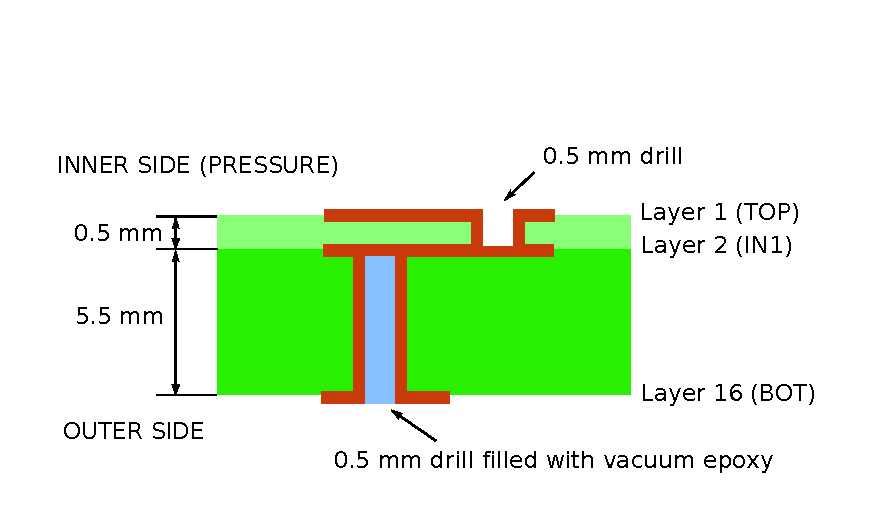
\includegraphics[width=.7\textwidth]{Stackup_feedthrough5.pdf}}
        \caption{\textit{Cross section of the PCB stackup}}
        \label{fig:ft:pcb}
    \end{center}
\end{figure}

We developed a small prototype that has one connector on each side and allows to take the signals of one full DICE-Board. It is designed with the same connector as the inner cables, so it can be directly connected to the DICE-Board pigtail. The prototype is shown in figure \ref{fig:ft:pcb2}.

\begin{figure}[ht]
  \centering
  \subfloat[\textit{Prototype PCB}]{%\label{fig:cabling:}
  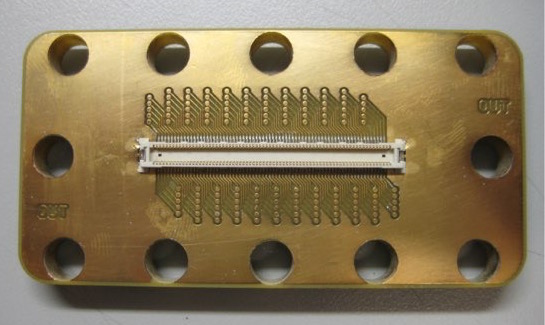
\includegraphics[height=0.35\textwidth]{IMG_0001.jpg}}   
  \hspace{10mm}             
  \subfloat[\textit{Flange for the PCB}]{%\label{fig:ad:ads7883}
  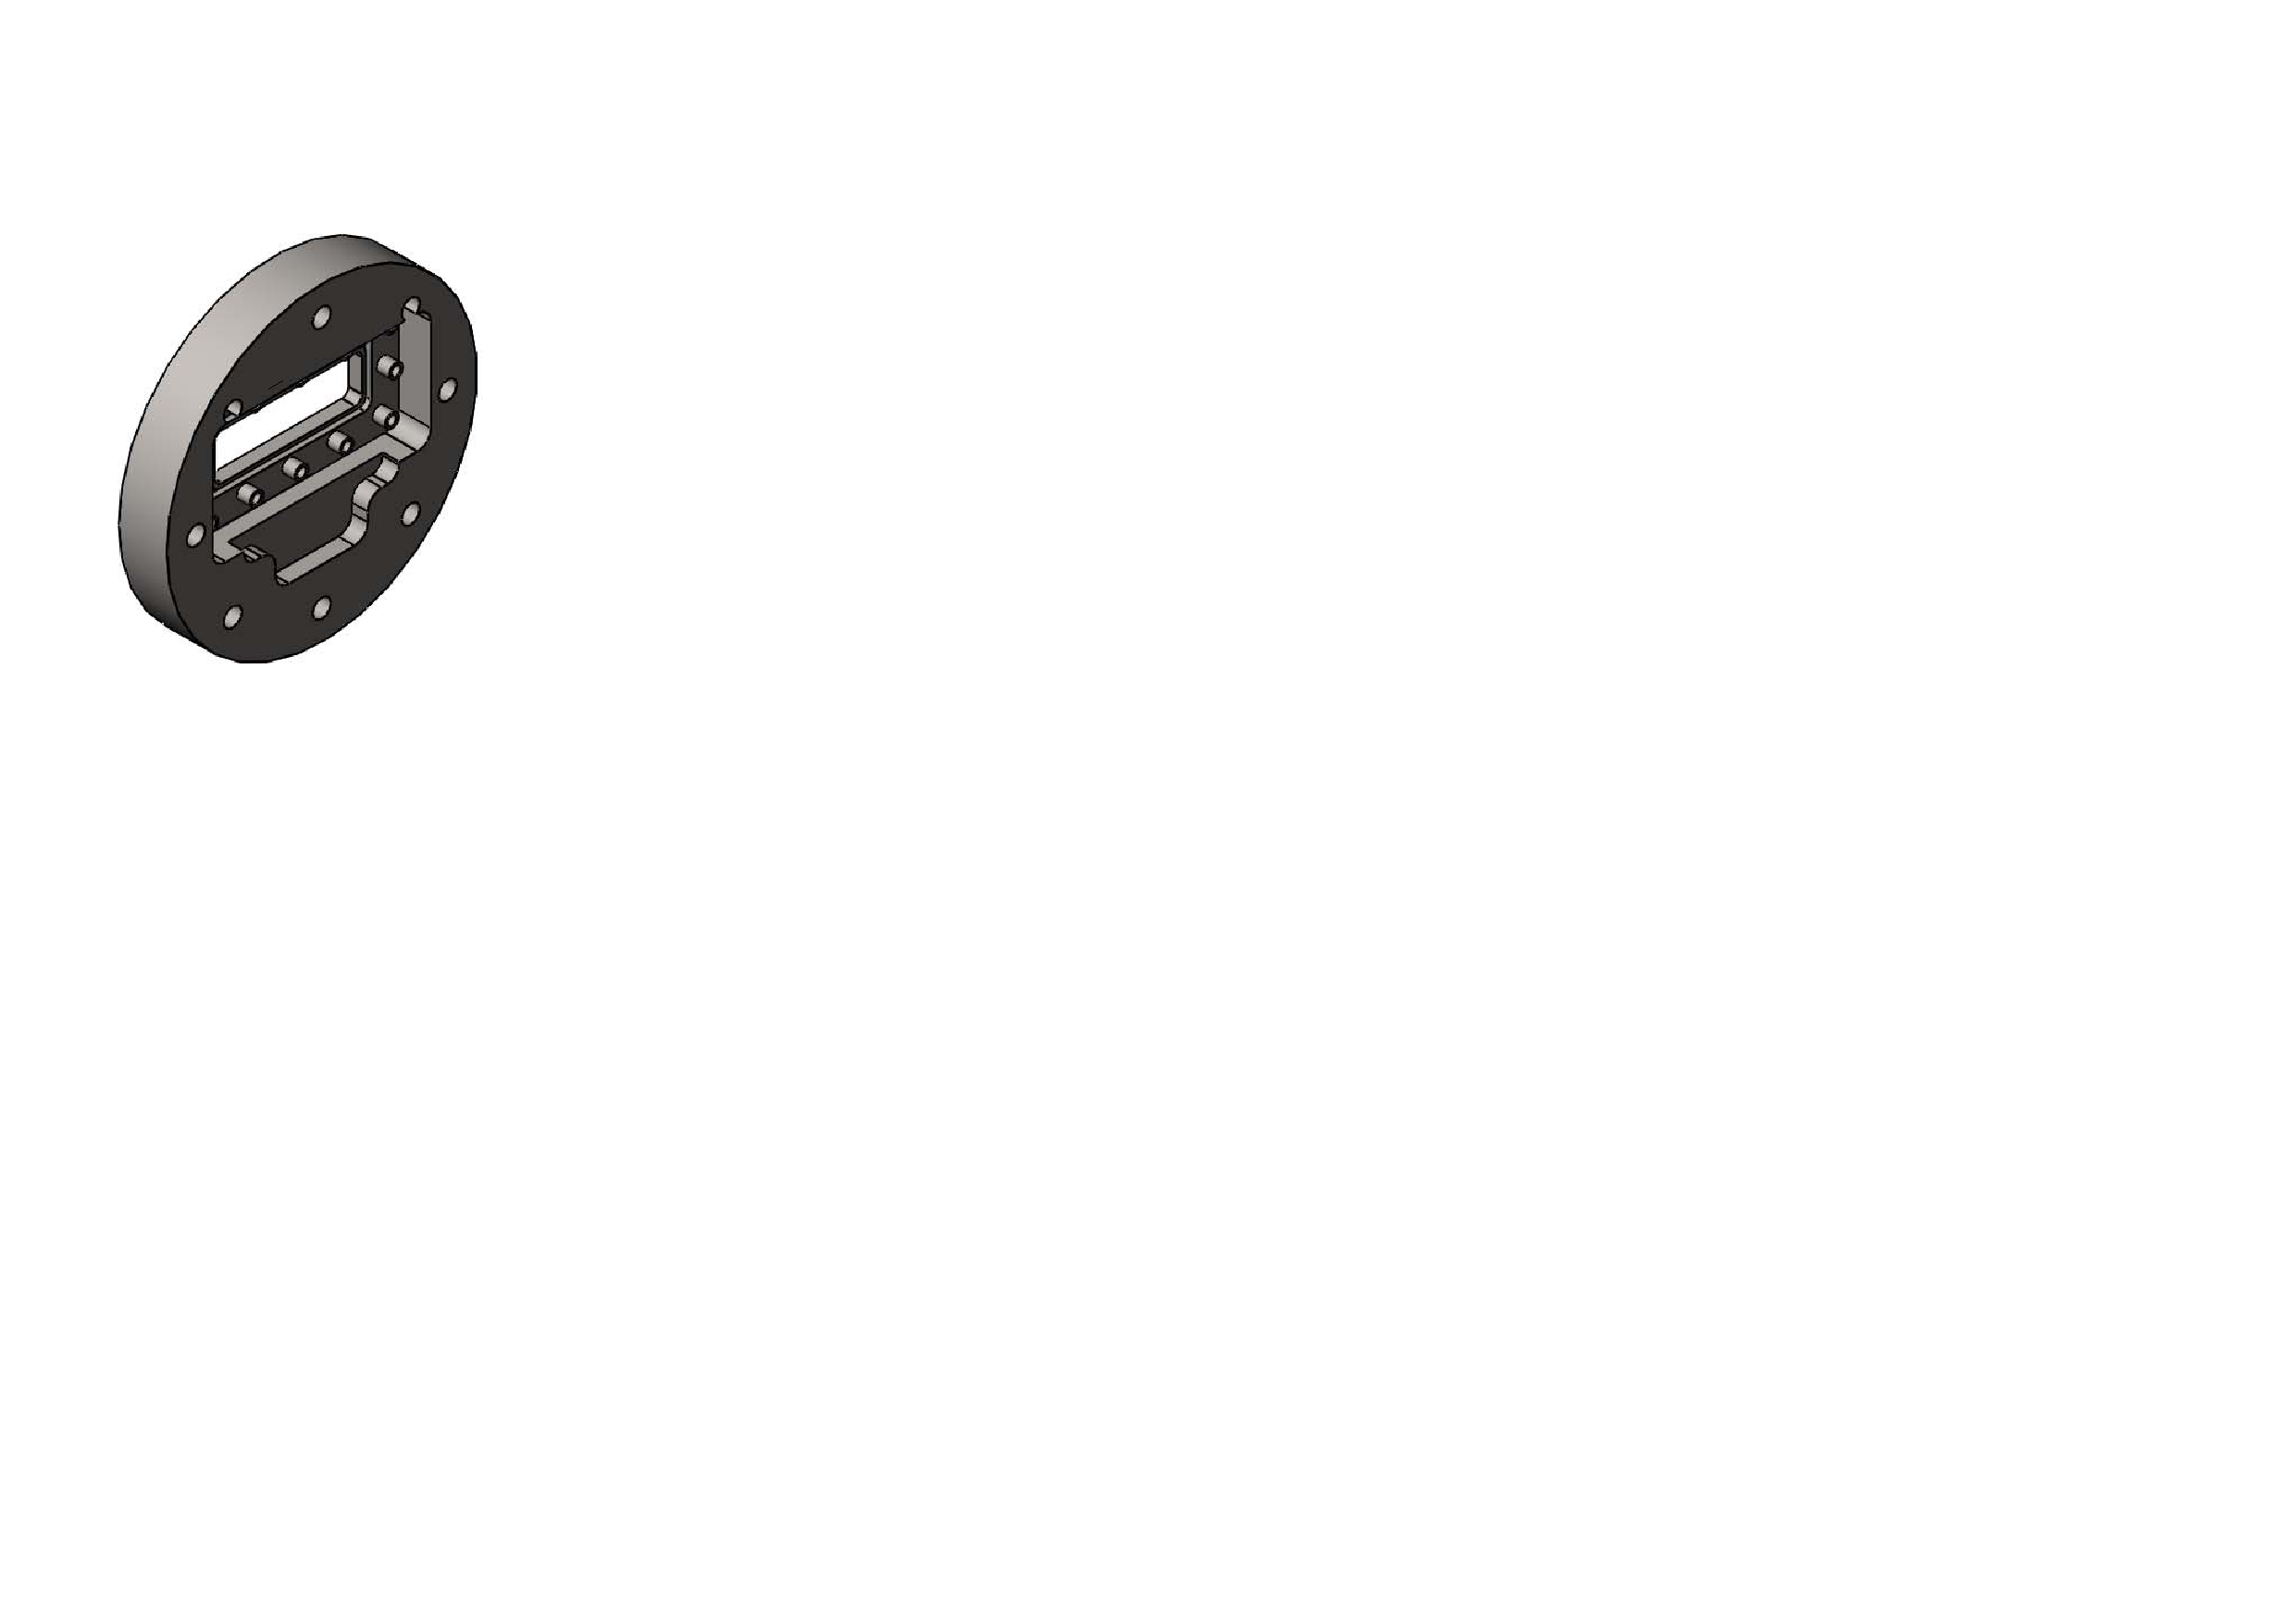
\includegraphics[height=0.35\textwidth]{FT_PCB2.pdf}}
  \caption{\textit{FR4 PCB feedthrough prototype}}
  \label{fig:ft:pcb2}
\end{figure}

The $6\ mm$ thickness of the design will hold more than $20\ bar$ of pressure, since standard FR4-class PCB materials have very good mechanical characteristics. In case we modify the design for a bigger shape, some stainless steel reinforcements will be enough. This feedthrough is quite cheap, because the materials and procedures used are standard on PCB production, while the only complicated parameter is the board thickness.

Using Ar at 20 bar pressure we measured a leak rate of $\sim10^{-2}~n mol/s$. The designed leak rate for NEW is $<10~g/year\ \longrightarrow\ 2.3~nmol/s$ for Xe; so as the Ar molecule is smaller than Xe, the feedthrough leak rate should be even lower for Xe.

\subsection{NEW FR4 PCB feedthrough}

For NEW the design includes $6$ connectors for DICE-Boards, with the same PCB stackup than the prototype. To make easier the sealing with the flange the new feedthroughs are round shaped, and also a stainless steel reinforcement plate is added at the back side, as shown in figure \ref{fig:big1}.

\begin{figure}[ht]
  \centering
  \subfloat[\textit{Feedthrough design (FR4 PCB and flange)}]{\label{fig:big1}
  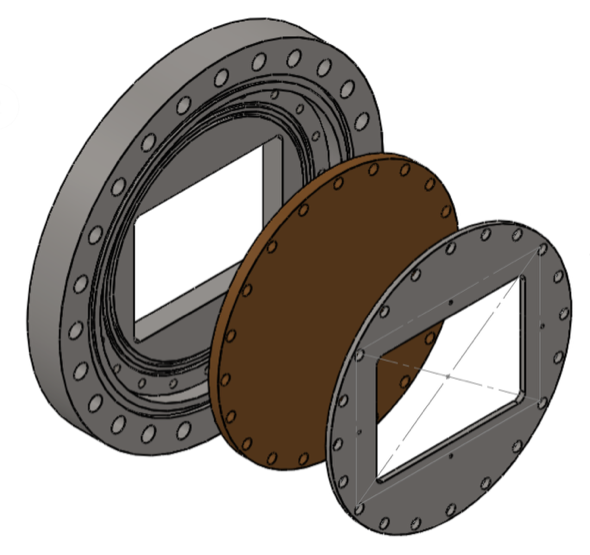
\includegraphics[height=0.35\textwidth]{FTBIG.png}}   
  \hspace{10mm}             
  \subfloat[\textit{NEW adapter for 5 feedthrough PCBs}]{\label{fig:big2}
  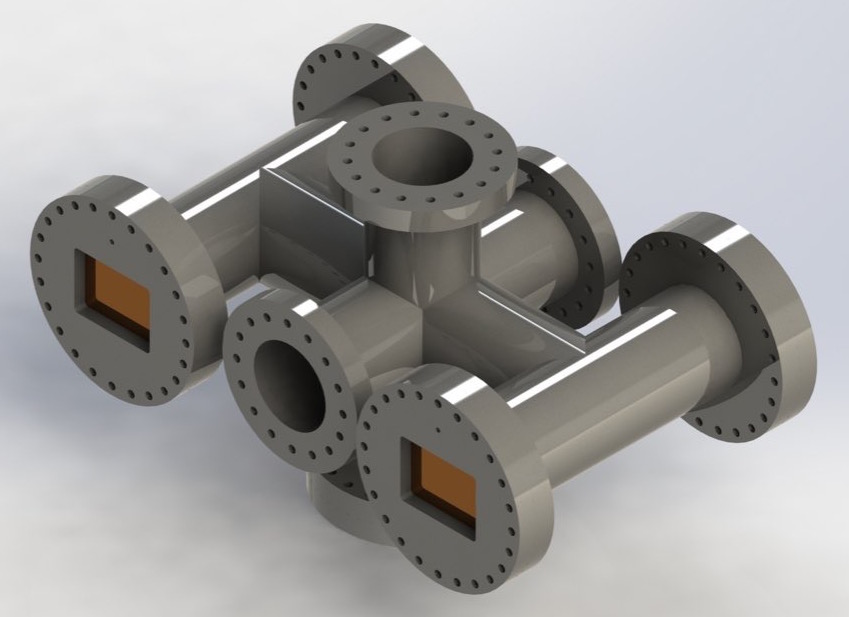
\includegraphics[height=0.35\textwidth]{5-FT_TP.jpg}}
  \caption{\textit{FR4 PCB feedthrough design for NEW}}
  %\label{fig:ft:pcb2}
\end{figure}

The flange union with the PCB has a double elastomer gasket, which is butyl rubber o-rings. For the sealing between the flange and the pipe we are using metal gaskets. As it is shown in figure \ref{fig:big2} we have designed a multi-port adapter for the vessel. This way we can  place the 5 feedthroughs required for NEW, and also easily replace them if necessary. It has also two additional ports, one for gas flow and other one as spare.

The new feedthrough has been manufactured (as can be seen on figure \ref{fig:FTfinal}) and tested at 20 bar pressure of Ar, giving a leak rate of $6\cdot 10^{-3}~nmol/s$. As the designed leak rate for NEW is $<10~g/year\ \longrightarrow\ 2.3~nmol/s$, even using 5 feedthroughs we are very far away from the limit. 

\subsection{Adapter boards and cable supports}

As explained on section \ref{sec:DB}, we use 4 cables per DICE-Board to connect them from the feedthrough to the front-end boards. But in order to achieve the minimum size of the feedthrough, it only has one connector per DICE-Board. For this reason we need an adapter from the feedthrough connector to the 4 cable stack. We designed a 4-layer rigi-flex board, shown on figure\ref{fig:adapter}, which is a hybrid circuit board with rigid areas made of standard FR4, and flexible layers made of polyimide. This way we are able extend the interface between the feedthrough and the external cables.

\begin{figure}[ht]
  \centering
  \subfloat[\textit{Adapter board (rigi-flex)}]{\label{fig:adapter}
  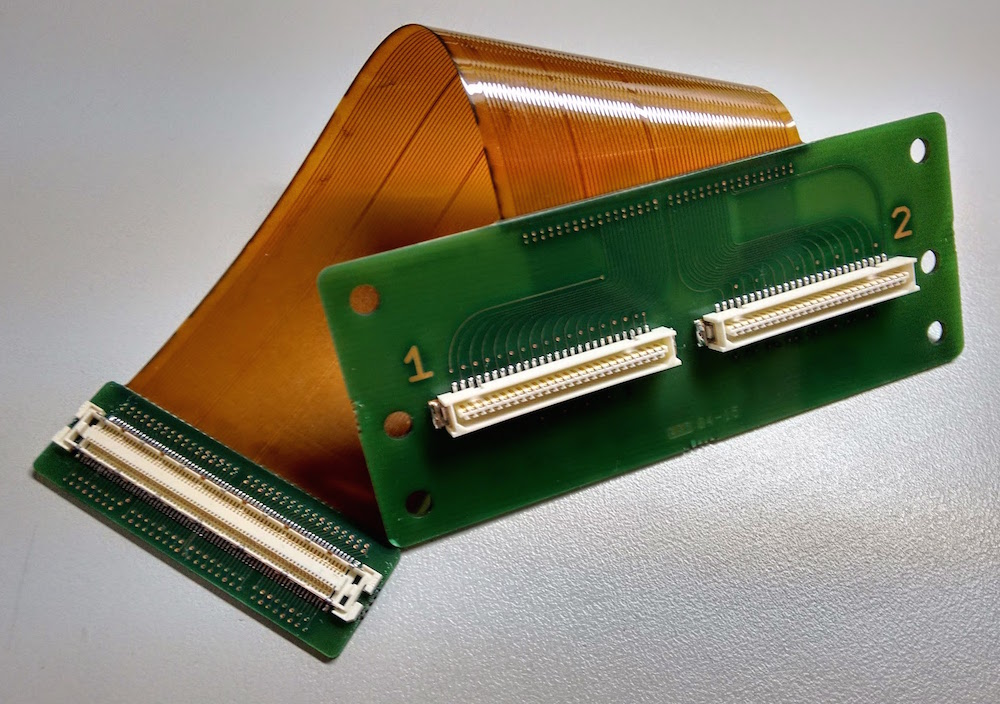
\includegraphics[height=0.32\textwidth]{Adapter.jpg}}   
  \hspace{10mm}             
  \subfloat[\textit{Feedthrough and flange}]{\label{fig:FTfinal}
  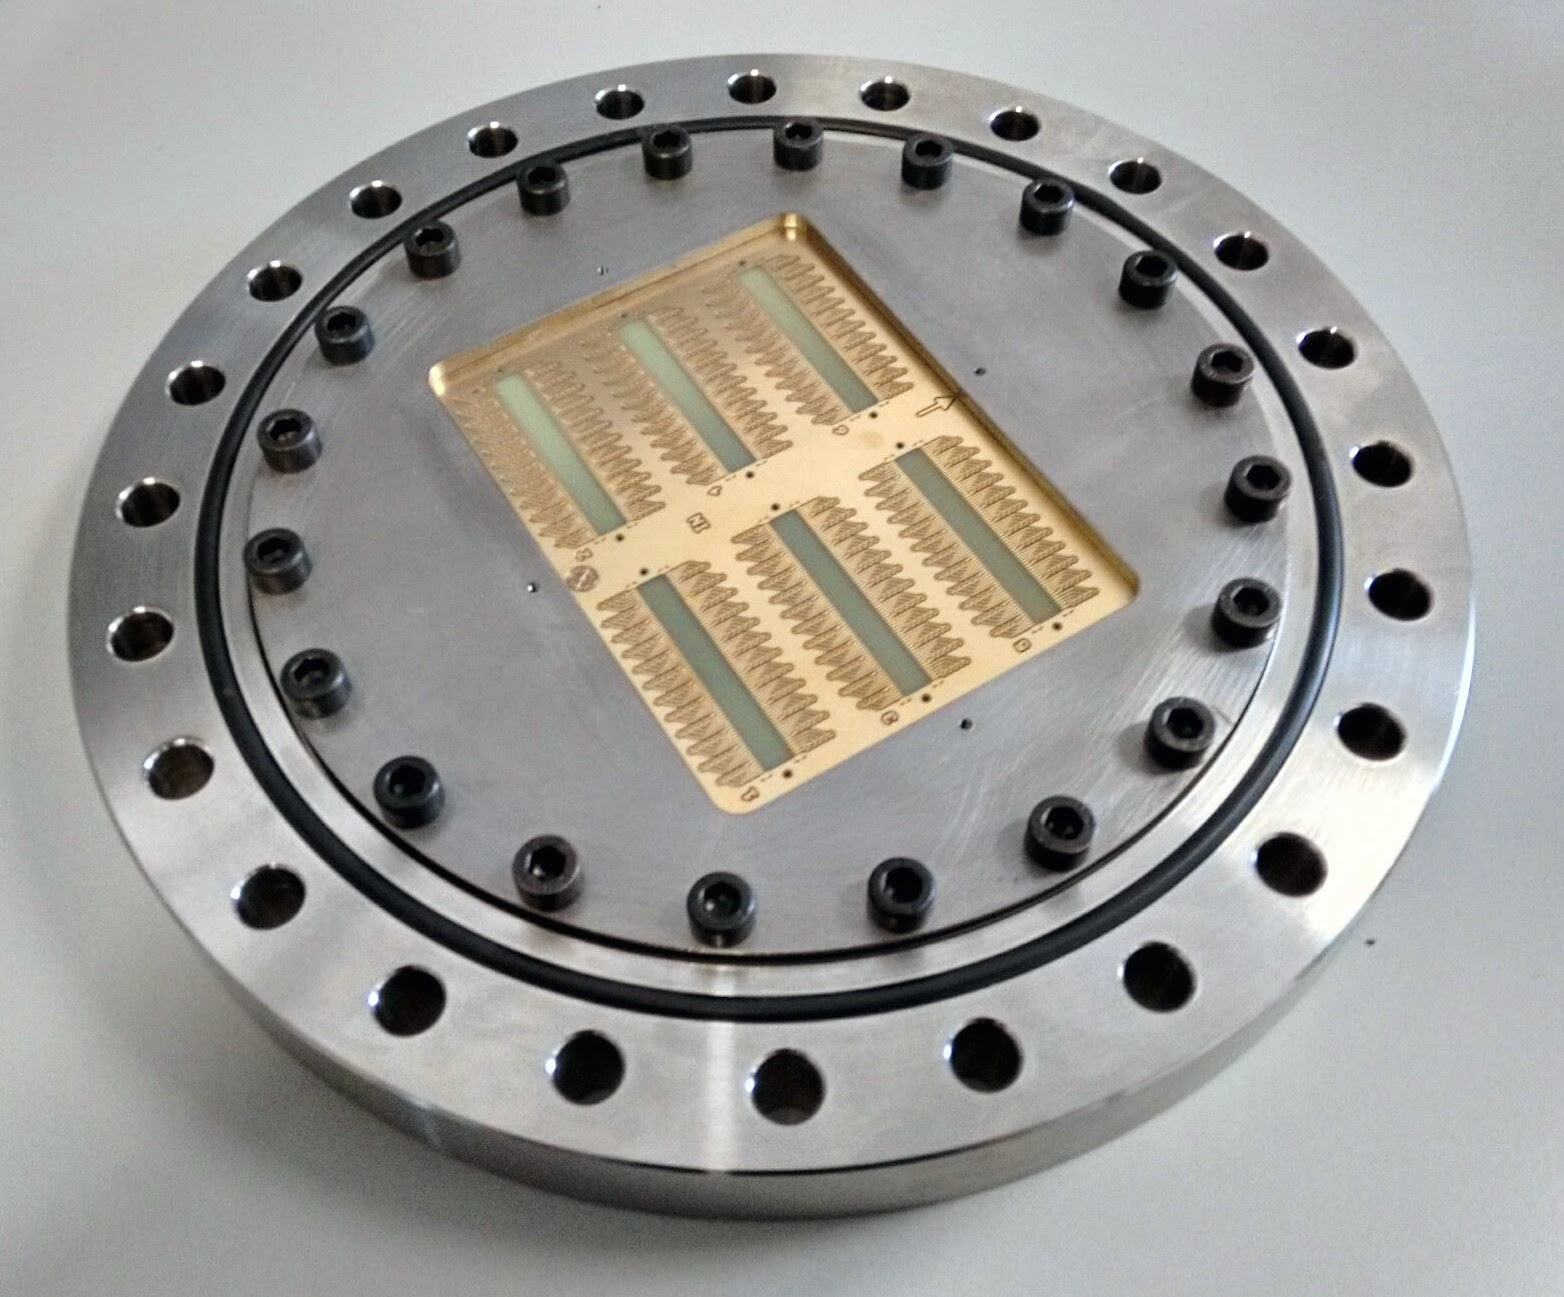
\includegraphics[height=0.32\textwidth]{FT_final.jpg}}
  \caption{\textit{Adapter board and feedthrough already manufactured}}
  %\label{fig:ft:pcb2}
\end{figure}

To fix the adapter boards to the feedthrough we designed a structure of 6 columns attached to the flange, and 3 clamps to keep the connectors on its place. On figure \ref{fig:mockup} is shown the mockup of this structure, done with a PLA 3D printer. As can be seen the adapter boards form an hexagon around the center of the feedthrough, which allows the easy connection of the cables. Finally, on figure \ref{fig:render} there is a render picture of the final feedthrough assembly.

\begin{figure}[ht]
  \centering
  \subfloat[\textit{Adapter boards support mockup}]{\label{fig:mockup}
  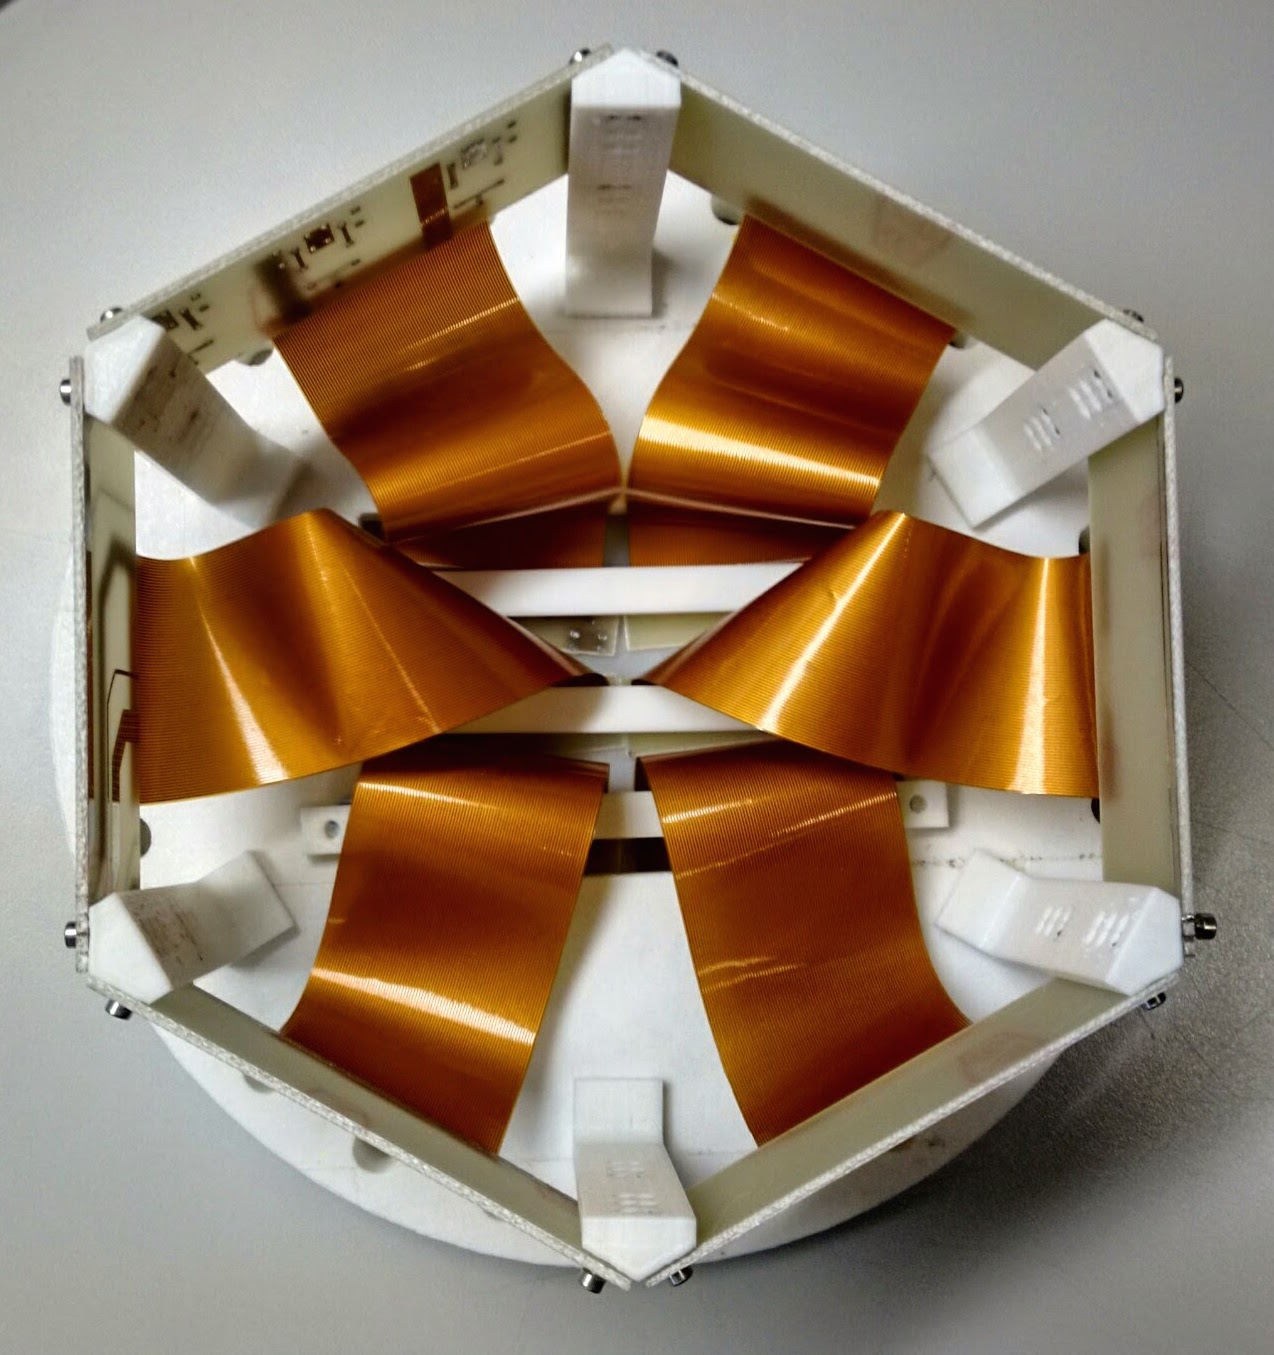
\includegraphics[height=0.38\textwidth]{Support.jpg}}   
  \hspace{10mm}             
  \subfloat[\textit{Feedthrough distribution}]{\label{fig:render}
  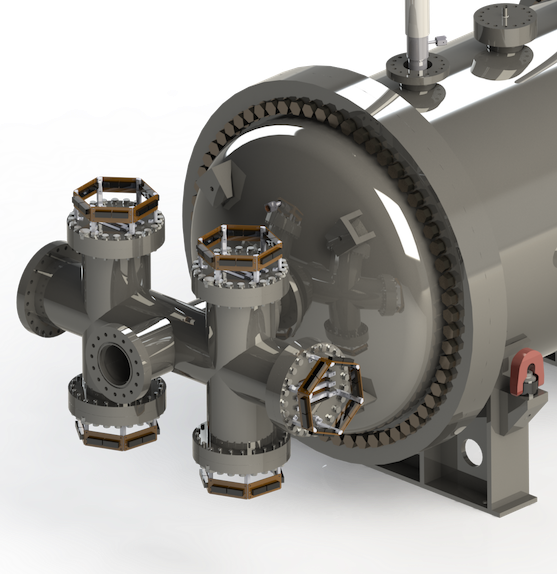
\includegraphics[height=0.38\textwidth]{FT_render.png}}
  \caption{\textit{Feedthrough details}}
  \label{fig:ft:mockuprender}
\end{figure}


%%%%%%%%%%%%%%%%%%%